

\begin{frame}[allowframebreaks]{Objectives}
		
    \begin{enumerate}[\textbullet]
        \item Write a class for the EnKF in C++, inspired by the EnKF written in Python (FilterPy); Test the algorithm.
        \item To read the following article :
        \begin{itemize}
            \item Fundamentals Of Building Performance Simulation By Beausoleil-Morrison
        \end{itemize}
        
    \item Understand the heat equation and what are the phenomena involved in the modification of the temperature of a building (conduction, convection, radiation).
    \item Write the mathematical problem to be solved if we want to simulate an office then realize the simulation using Feel++ toolboxes.
    \item Introduce data assimilation using the sensor and correct the simulation.
    \end{enumerate}
\end{frame}




\begin{frame}{Introduction to data assimilation}
Data assimilation is widely used in:
\begin{enumerate}[\textbullet]
       \item weather forecasting
       \item ocean simulation
\end{enumerate}	 
      The main idea of computational data assimilation is to combine:
\begin{enumerate}[\textbullet]
       \item a model
       \item some observations
\end{enumerate}	 
The best estimation:
$$x^a=Lx^b+Ky^0$$
with $x^a$ the analyzed state, $x^b$ the state of the model and $y^0$ the observations.
\end{frame}
\subsection{Theory}
   
\begin{frame}{Kalman filter in multi-dimensional case}
   Now that we have explained the method for finding $x^a$ let's try to generalize our formula in a \textbf{multi-dimensional case}.

   $$\left\{\begin{aligned}
     &x^a=(I-KH)x^b+Ky^0=x^b+K(y^0-H(x^b)) \\
           &K=BH^T(HBH^T+R)^{-1} \\
    \end{aligned}\right.$$
   With $K$ the gain or weight matrix.
   \begin{figure}[H]
       \pgfimage[width=0.4\linewidth]{images/enkf/schema_kalman_filter.png}
       \caption{Kalman Filter}
   \end{figure}
\end{frame}
\begin{frame}[allowframebreaks]{Ensemble Kalman Filter}
   \noindent The ENKF method consists in using the Kalman filter method in high dimension and compare P by a set of states $x_1,x_2,..,x_{m}$. So we can approximate the moments of the error by the moments of the sample.
For all the samples, we have:
$$x_i^a=x_i^f+K[y-h(x_i^f)]$$
with $h(x_i^f)$ the observation operator.
\newline \noindent To begin with we can estimate the
forecast error covariance matrix as:
$$P^f=\frac{1}{m-1}\sum_{i=1}^{m}(x_i^f-\bar{x}^f)(x_i^f-\bar{x}^f)^T~~with~~\bar{x}^f=\frac{1}{m}\sum_{i=1}^{m}x_i^f .$$ 
\noindent We can factorized the forecast error covariance matrix by:
$$P^f=X_f X_f^T$$
where $X_f$ is an $n \times m$ matrix whose columns are the normalized anomalies or normalized perturbations,
$$[X_f]_i=\frac{x_i^f-\bar{x}^f}{\sqrt{m-1}}$$

\noindent We can also define the Kalman gains: 
$$K=P^f H^T(HP^f H^T+R)^{-1}$$

\noindent In addition, we have:
$$
\bar{x}^a=\frac{1}{m}\sum_{i=1}^mx_i^a~~,~~~~[X_a]_i=\frac{x_i^a-\bar{x}^a}{\sqrt{m-1}}. $$
\newline \noindent We can write the covariance matrix of the analysis errors as:
$$P^a=(I_n-KH)P^f(I_n-KH)^T+KRK^T=(In-KH)P^f.$$
\noindent Add a disruption to the observation: $y\rightarrow y_i+\bar{u_i}$ where $u_i$ is drawn from the Gaussian distribution $u_i \sim \mathcal{N}(0,R)$
\newline the innovation perturbations as :
$$[Y_f]_i=\frac{Hx_i^f-u_i-H\bar{x}^f+\bar{u}}{\sqrt{m-1}}.$$
\noindent Finally we can modify the posterior anomalies:
$$X_i^a=X_i^f-KY_i^f=(I_n-KH)X_i^f+\frac{K(u_i-\bar{u})}{\sqrt{m-1}}.$$
\end{frame}
\begin{frame}{Ensemble Kalman Filter}
    \begin{figure}[H]
		\pgfimage[width=0.85\linewidth]{images/enkf/algorithm.png}
	\end{figure}
\end{frame}
\begin{frame}[allowframebreaks]{Comparing Cpp results with Python}
\begin{minipage}{0.4\hsize}
			\centering
	\begin{figure}[H]
		\pgfimage[width=0.9\linewidth]{images/enkf/result.png}
		\caption{Visualization of the model and observations (Initial condition: $X_0=(-10.,-10.,25.) $ )}
	\end{figure}
		\end{minipage} \quad
		\begin{minipage}{0.5\hsize}
			\begin{itemize}
    \item $(\sigma, r, b)=(12.,6.,12.)$ for observation
    \item $(\sigma, r, b)=(10.,6.,10.)$ for the model
    \item $$P=\begin{pmatrix}
            0.1 & 0. & 0. \\
            0. & 0.1 & 0. \\
            0. & 0. & 0.1 \\
            \end{pmatrix}
            Q=\begin{pmatrix}
            0.1 & 0. & 0. \\
            0. & 0.1 & 0. \\
            0. & 0. & 0.1 \\
            \end{pmatrix}$$
            \newline
            $$R=\begin{pmatrix}
            0.01 & 0. & 0. \\
            0. & 0.01 & 0. \\
            0. & 0. & 0.01 \\
            \end{pmatrix}.$$ 
    \end{itemize}
		\end{minipage}
		
\newpage
\centering
	\begin{figure}[H]
		\pgfimage[width=1\linewidth]{images/enkf/result_filterpy.png}
		\caption{Result with Filterpy}
	\end{figure}

\newpage
\centering
	\begin{figure}[H]
		\pgfimage[width=1\linewidth]{images/enkf/result_cpp.png}
		\caption{Result with Cpp}
	\end{figure}

\end{frame}
\subsection{Integrate data assimilation to Feel++}
\begin{frame}[allowframebreaks]{The context}
\begin{itemize}
    \item Our goal is to make the thermal simulation of an office in the university of Strasbourg in which we have 10 sensors to measure the temperature.\\
    \item We want to apply data assimilation and use our sensors to correct the temperature of the room.
\end{itemize}

\begin{minipage}{0.48\linewidth}
    \begin{figure}
        \centering
        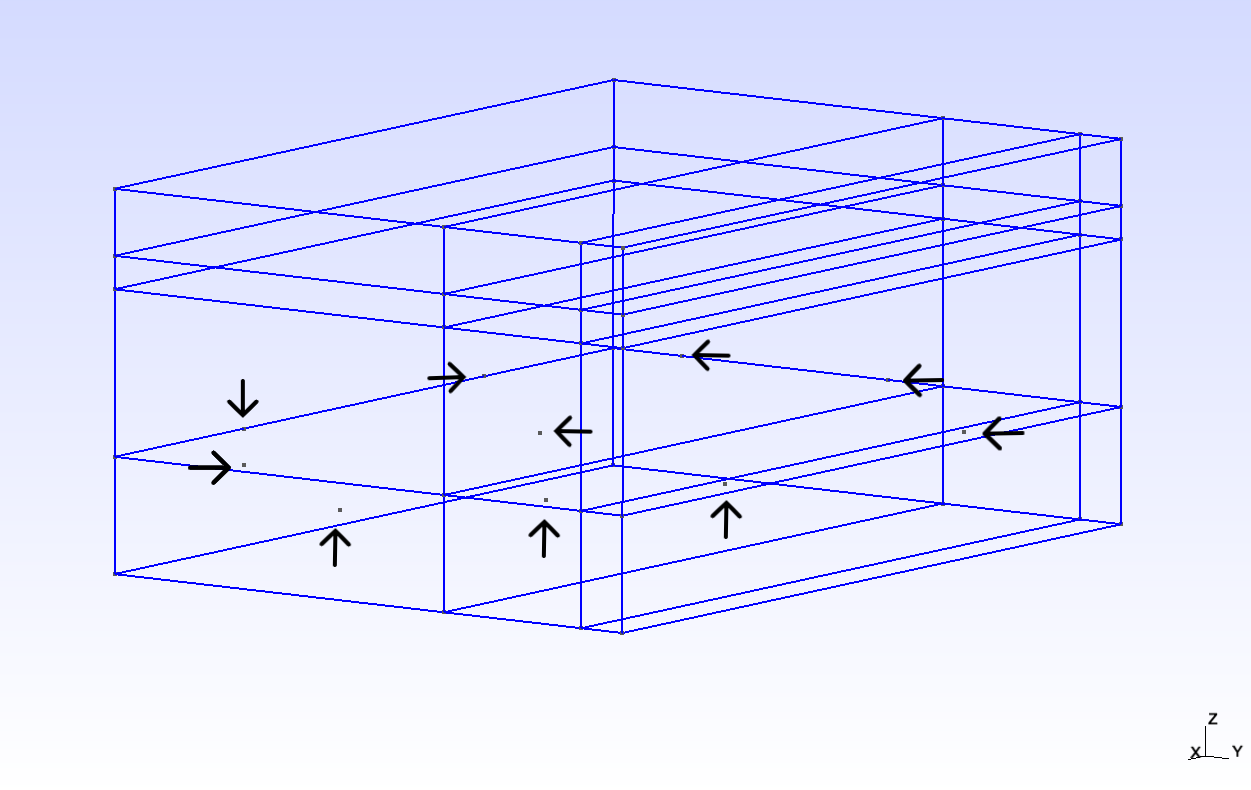
\includegraphics[width=\linewidth]{"images/enkf/Maillage_1.png"}
        \caption{Mesh of the office that we will use for the simulation.}
    \end{figure}
\end{minipage} \;
\begin{minipage}{0.48\linewidth}
    \begin{figure}
        \centering
        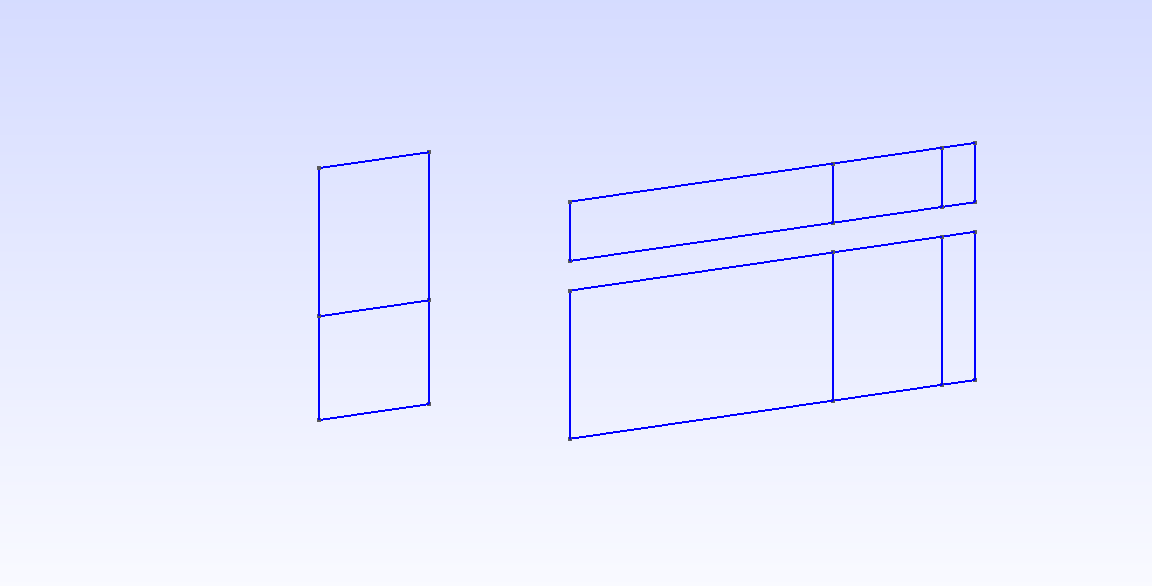
\includegraphics[width=\linewidth]{"images/enkf/Maillage_2.png"}
        \caption{Visualization of windows and door in the mesh.}
    \end{figure}
\end{minipage}
\newpage
\begin{itemize}
    \item Heat equation with convective effects\\
    $$\rho C_p((\frac{\partial T}{\partial t})+u \cdot \nabla T)-\nabla \cdot (k \nabla T)=Q$$
    Which is completed with boundary conditions and initial value.
    \newline
    \newline
\renewcommand{\arraystretch}{2}
\begin{tabular}{|R{2cm}|C{2.5cm}|L{2.5cm}|L{2.5cm}|}
\hline
$\rho$ & Air density & $Kg.m^
{-3}$ & 1.125  \\[0.5cm]
\hline
$C_p$ & Specific heat & $J/KgK$ & 1004 \\[0.5cm]
\hline
$k$ & Conductivity & $W/mK$ & 0.025  \\[0.5cm]
\hline
$u$ & Fluid velocity & $m.s^{-1}$ & unknown \\[0.5cm]
\hline
\end{tabular}
\newpage
\item Equation of the air motion (Navier-Stokes).
 $$\left\{\begin{aligned} 
        &\rho (\frac{\partial u}{\partial t}+u\cdot \nabla u)-\nabla \cdot (\mu \nabla u)+\nabla P =-\rho_0 \beta(T-T_{ref})g\\
        &\nabla . u=0 \\
    \end{aligned}\right.$$
\renewcommand{\arraystretch}{2}
\begin{tabular}{|R{1cm}|C{5cm}|L{1.5cm}|L{1.5cm}|}
\hline
$\rho$ & fluid density & $Kg.m^
{-3}$ & 1.125 \\[0.7cm]
\hline
$u$ & fluid velocity & $m.s^{-1}$ & unknown \\[0.7cm]
\hline
$\beta$ & coefficient of thermal expansion & $K^
{-1}$ &  0.0034 \\[0.7cm]
\hline
$\mu$ & dynamic viscosity & $Pa.s$ & $1.81e^{-5}$\\[0.7cm]
\hline
$g$ & gravitational acceleration & $m.s^{-2}$ & $9.8$\\[0.7cm]
\hline
\end{tabular}

\newpage
\item Heat equation without convective effects\\
    $$\rho C_p(\frac{\partial T}{\partial t})-\nabla \cdot (k \nabla T)=Q$$
    Which is completed with boundary conditions and initial value.
    \newline
    \newline
\renewcommand{\arraystretch}{2}
\begin{tabular}{|R{2cm}|C{2.5cm}|L{2.5cm}|L{2.5cm}|}
\hline
$\rho$ & Air density & $Kg.m^
{-3}$ & 1.125  \\[0.5cm]
\hline
$C_p$ & Specific heat & $J/KgK$ & 1004 \\[0.5cm]
\hline
$k$ & Conductivity & $W/mK$ & 0.025  \\[0.5cm]
\hline
\end{tabular}
\end{itemize}
\newpage
\begin{minipage}{0.30\linewidth}
    \begin{figure}
        \centering
        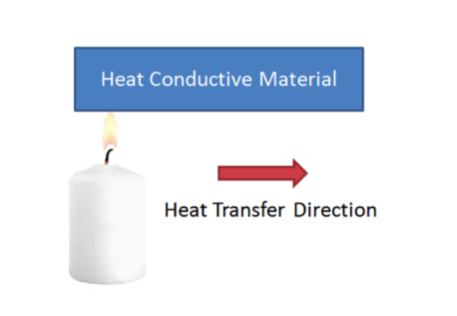
\includegraphics[width=1.2\linewidth]{images/enkf/conduction.png}
        \caption{Conduction}
    \end{figure}
\end{minipage} \;
\begin{minipage}{0.30\linewidth}
    \begin{figure}
        \centering
        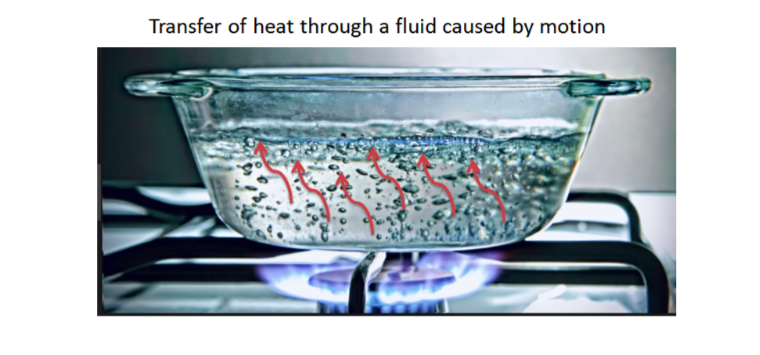
\includegraphics[width=1.2\linewidth]{images/enkf/convection.png}
        \caption{Convection}
    \end{figure}
\end{minipage}
\begin{minipage}{0.35\linewidth}
    \begin{figure}
        \centering
        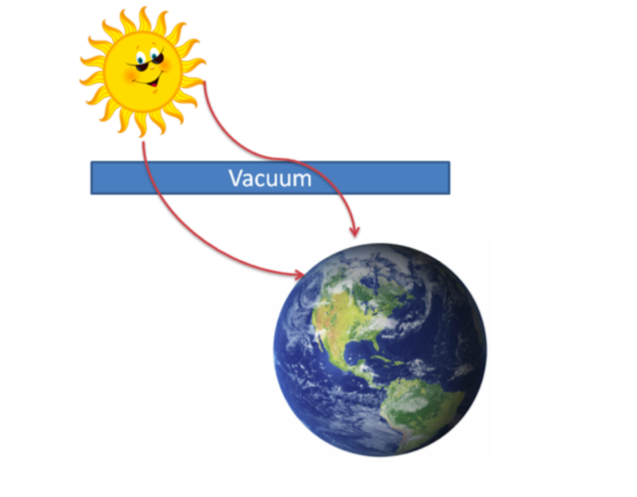
\includegraphics[width=1.2\linewidth]{images/enkf/radiation.png}
        \caption{Radiation}
    \end{figure}
\end{minipage}

\end{frame}
\begin{frame}[allowframebreaks]{Simulation}
\begin{minipage}{0.47\linewidth}
    \begin{figure}
        \centering
        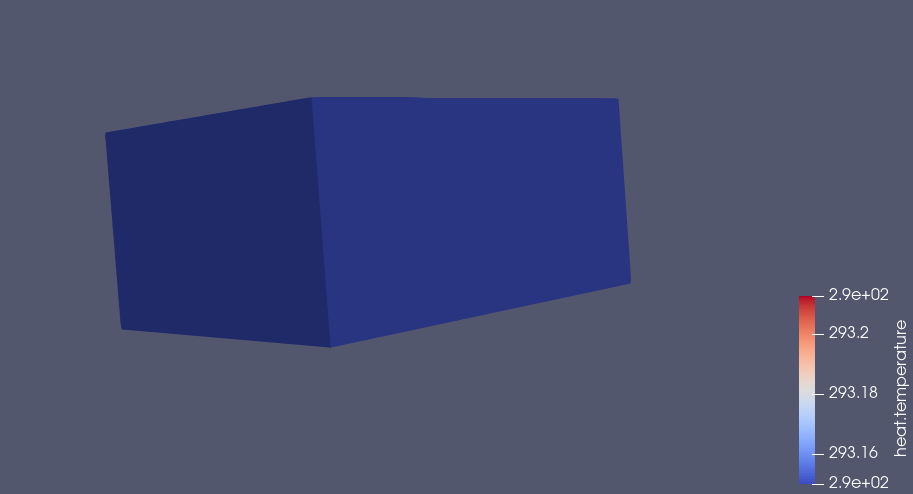
\includegraphics[width=\linewidth]{"images/enkf/sim_1.png"}
        \caption{Visualization of the simulation made with the toolbox heat (Initial condition ) .}
    \end{figure}
\end{minipage} \;
\begin{minipage}{0.48\linewidth}
    \begin{figure}
        \centering
        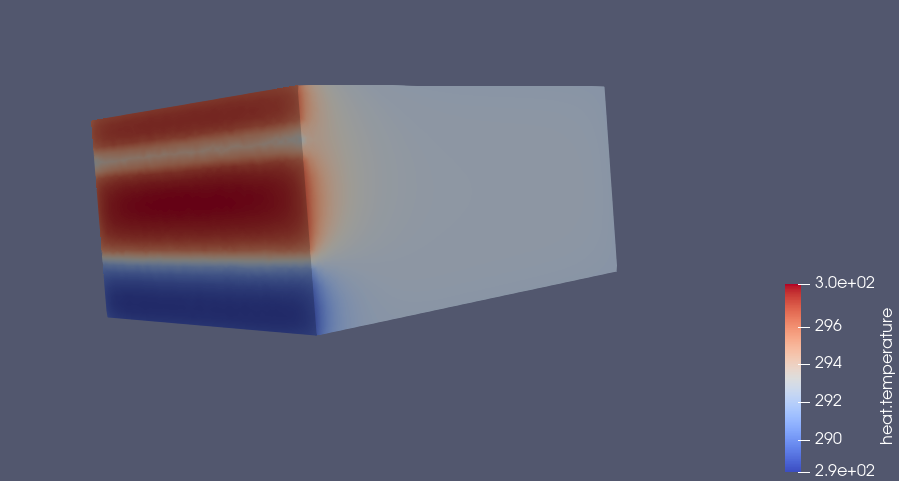
\includegraphics[width=\linewidth]{"images/enkf/sim_2.png"}
        \caption{Visualization of the simulation made with the toolbox heat (1 hour) .}
    \end{figure}
\end{minipage}
\begin{itemize}
    \item For this simulation we do not consider the convection .
\end{itemize}

\end{frame}
    
\begin{frame}[allowframebreaks]{Including data assimilation to our simulation}
\begin{minipage}{1\linewidth}
    \begin{figure}
        \centering
        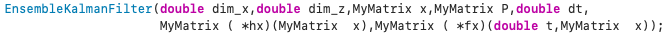
\includegraphics[width=\linewidth]{"images/enkf/enkf.png"}
    \end{figure}
\end{minipage}
Ensemble Kalman Filter class:
\begin{itemize}
    \item the dimension of our model;
    \item the dimension of the vector containing our observations;
    \item a vector X which will represent the initial state for our model;
    \item the matrix P ;
    \item our time step dt. 
    \item a function \text{hx};
    \item a function \text{fx}.

\end{itemize}
\newpage
The delicate part to realize the data assimilation was to create the fx function.

	\begin{figure}[H]
		\pgfimage[width=0.6\linewidth]{images/enkf/Maillage_rayon.png}
		\caption{Mesh with radius on the sensors}
	\end{figure}


\end{frame}




